\section{PopCoins}

\subsection{User Interface}

\begin{figure}[!h]
    \centering
    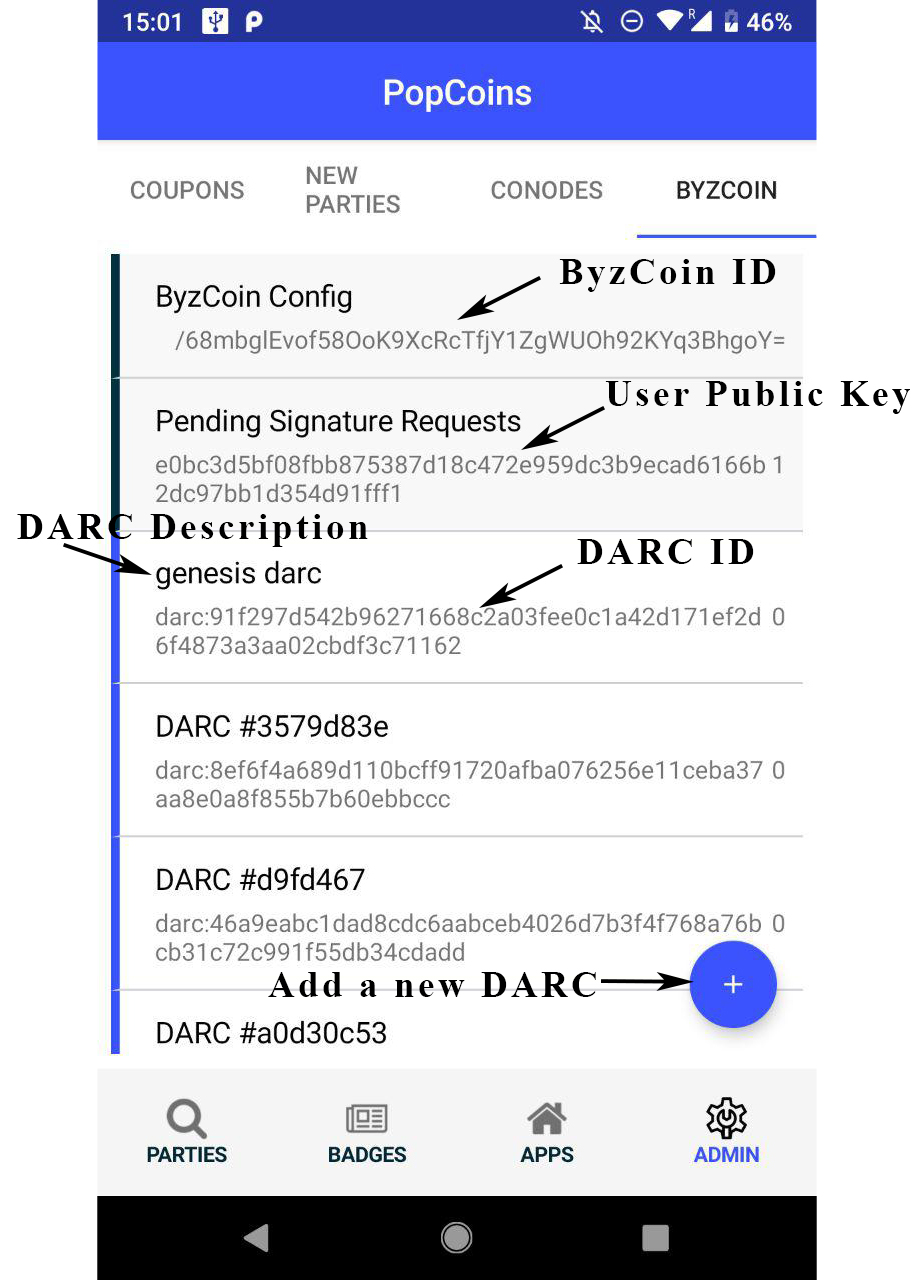
\includegraphics[height=1.4\linewidth]{Illustrations/screen_byzcoinmenu.jpg}
    \caption{\textit{ByzCoin} menu in \textit{PopCoins}}
\end{figure}

\subsubsection{ByzCoin main page}

\paragraph{}

\textit{ByzCoin} main page in \textit{PopCoins}, situated inside the Admin panel, is built around two lists:

\begin{itemize}
    \item The first list is of fixed size, and is composed of two elements which lead to sub-menus. The first element is the \textit{ByzCoin} config, and leads to a description of it. The second element is only a stub in the current state of the project. Its a a menu meant to contain signature requests for the multi-signature implementation. This first list is differentiated from the second one through the use of a different colour on the side, declared in CSS as:\newline
    \crule[night-dark] \textit{night-dark}, RGB = {2, 49, 65}\newline
    The colour of the background is also a little bit darker:\newline
    \crule[background-dark] \textit{background-dark}, RGB = {248, 248, 248}
    \item The second list is dynamic, and shows the different \textit{DARC} locally saved by the user. When the user taps a \textit{DARC}, it leads to a page with its complete description. This list is identified  by the colour:\newline
    \crule[accent-dark] \textit{accent-dark}, RGB = {58, 83, 255}
\end{itemize}

\paragraph{}

There is also a floating blue button, with a white + cross, floating in the bottom-right corner of the page, and which is used to add a new \textit{DARC}. The second list is fully scrollable in the event it exceeds screen size, which allows the elements a the first list to be always visible.

\subsubsection{Adding a new DARC}

\paragraph{}

Upon clicking on the white + button, a dialog pops-up in the app and presents the two different options available to the user:

\begin{figure}[!h]
    \centering
    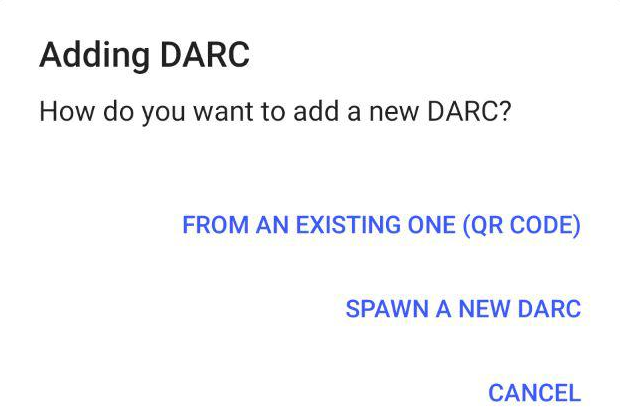
\includegraphics[height=0.45\linewidth]{Illustrations/screen_adddarc_cropped.png}
    \caption{\textit Dialog offering to add a new \textit{DARC} in \textit{PopCoins}}
\end{figure}

\begin{itemize}
    \item From an existing one, using a QR Code. This option will open up a QR Code scanner the user can use in order to read a QR Code generated from \textit{PopCoins} app on another device. The whole scanning process is described in \hyperref[subsection53]{sub-section 5.3}. If the user scans the QR Code of a \textit{DARC} A that has the same \textit{BaseID} as a \textit{DARC} B stored locally, \textit{DARC} A will replace \textit{DARC} B if and only if its version number is strictly superior to B's; otherwise, A gets dropped.
    \item Spawning a new \textit{DARC}. In that case, \textit{PopCoins} will automatically generate the \textit{DARC}, with the current user as its owner, and the string "\textit{DARC \#}" followed by a random 8-digits hexadecimal number as description (for the reasons explained in \hyperref[subsection413]{sub-section 4.1.3}). In the background, the app will check that the user has at least one \textit{DARC} on which he has the right to \textit{spawn:darc}, otherwise the operation will fail. If the user has multiple \textit{DARC} with the \textit{spawn:darc} right, the first one in the list will be used for the transaction.
\end{itemize}

\subsubsection{DARC description page}

\paragraph{}

The \textit{DARC} description page is composed of a single, scrollable list that shows all of its information. It ends is a dynamically generated list if its rules, identified by the action in the title and the linked expression in the content of the list element. On top, there is a button to go back to the \textit{ByzCoin} main page, a button to delete the \textit{DARC} from local memory (not from \textit{ByzCoin}!), and a button to generate the QR Code representation of the \textit{DARC}. In the bottom-right corner, there is a floating button containing a white + that allows the addition of new rules.

\paragraph{}

Whenever a rule is clicked, a dialog pops-up allowing the user to either delete the rule, or edit it. The rules \textit{\_sign} and \textit{invoke:evolve} cannot be deleted. The description of the \textit{DARC} can also be edited by the user the same way. In any case, for addition, edition or deletion, the user needs to have the \textit{invoke:evolve} right on the \textit{DARC}, as in the background, any change of that kind performs an evolution of the \textit{DARC}. If the evolution process fails, an error dialog appears and the change to the \textit{DARC} is cancelled.

\paragraph{}

The \textit{ByzCoin} config description page is very similar to the \textit{DARC} description page. There are only a few differences:

\begin{itemize}
    \item If no config is saved locally, the delete and share button are replaced by a + button that will allow to scan a config QR Code
    \item There is no possibility to either add, edit or delete config parameters. The user can only completely delete the config to load a new one
\end{itemize}

\begin{figure}[!h]
    \centering
    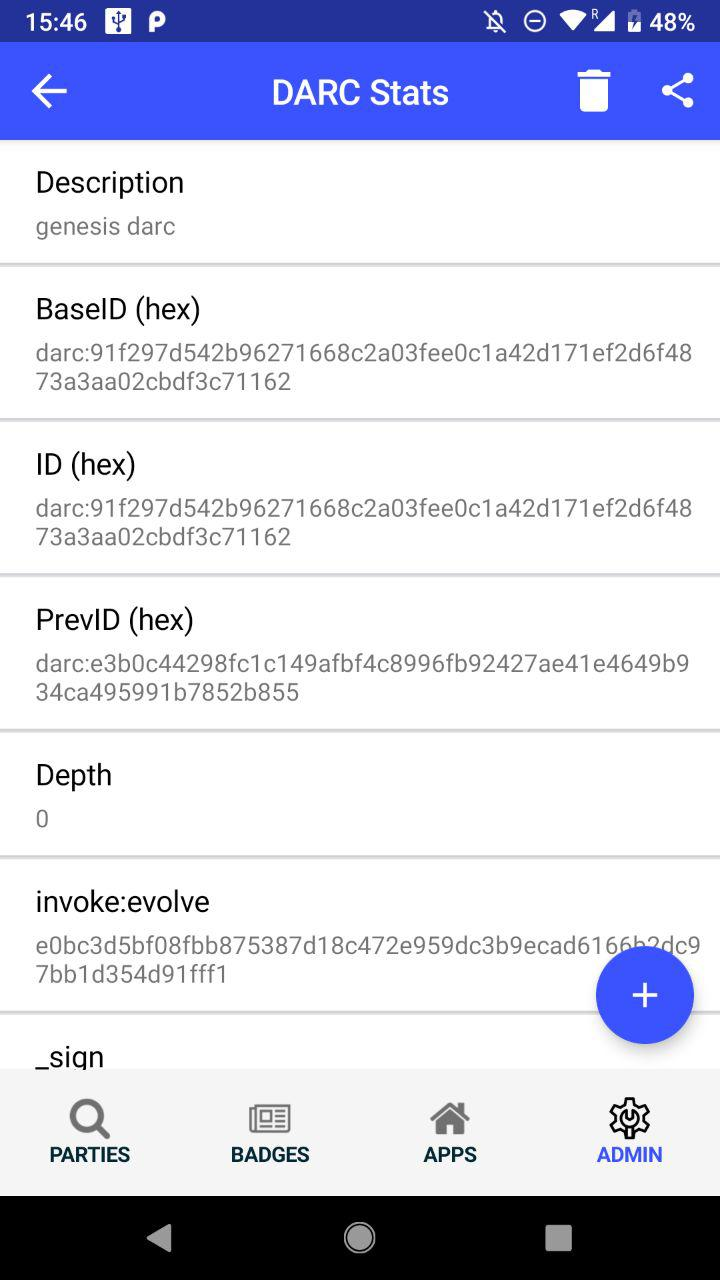
\includegraphics[height=0.8\linewidth]{Illustrations/screen_darcdesc.jpg}
    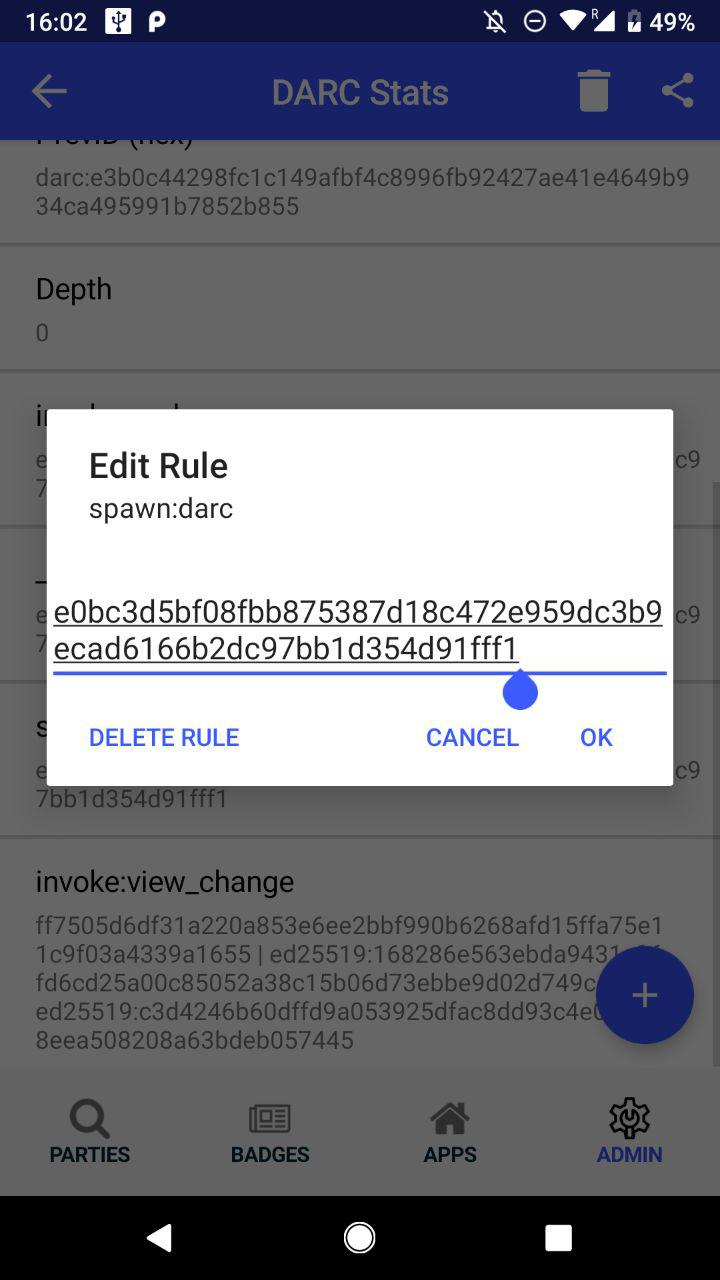
\includegraphics[height=0.8\linewidth]{Illustrations/screen_darceditrule.jpg}
    \caption{\textit \textit{DARC} description page in \textit{PopCoins}}
\end{figure}

\subsection{Local saves}

\paragraph{}

\textit{PopCoins} has to save some information inside the device's memory in order to keep it between two runs. Those saves are made in the form of JSON\footnote{\url{https://www.json.org/}} files, which locations are registered inside constants in the \textit{FilePaths.js} file. During this project, two new elements had to be saved by the application: the \textit{ByzCoin} config and the registered \textit{DARC}. As for the \textit{Conodes} and other user information, those saves are performed inside \textit{User.js}.

\paragraph{}

One of the main issues caused by saving in JSON format is that \textit{JavaScript} does not support well the stringification of \textit{Map()} objects, which are used to represent \textit{DARC} rules. In order to solve this issue, the solution that has been chosen is to create a temporary \textit{DARC} object during the saving process, that instead of a \textit{Map()} uses an \textit{Array()} of tuples. This allows an easy stringification while keeping the \textit{Map()} structure for \textit{DARC} objects, which is extremely practical for the usual operations on rules.

\subsection{Scanning objects}
\label{subsection53}

\paragraph{}

The main tool chosen for communication between devices connected to a same \textit{ByzCoin} instance is QR Code. This solution is extremely practical to share objects between mobile devices, and from computers to mobile devices. \textit{PopCoins} being the principal client aiming unexperienced users, this solution is particularly viable.

\paragraph{}

QR Code generation and scan were already implemented in the app before the start of this project, and used for example with the \textit{conodes}. It is built around the \textit{nativescript-barcodescanner} plugin for \textit{NativeScript}\footnote{\url{https://github.com/EddyVerbruggen/nativescript-barcodescanner}}. During this project, QR Code generation has been implemented for two new objects: \textit{ByzCoin} config and \textit{DARC}. As such, it is really easy for a user B to join the same \textit{ByzCoin} instance as user A: user A only has to generate QR Codes of his \textit{Conodes}, his config and eventually some of his locally saved \textit{DARC}.

\paragraph{}

The main challenge comes from the interaction via QR Code between BC Admin CLI and \textit{PopCoins}: both generate their QR Codes from JSON representations of the objects, but they do not represent those objects the same way. Decision has thus been taken that for the \textit{ByzCoin} config, the representation generated by BC Admin CLI would be the one used. It thus follows that in \textit{PopCoins}, a special parse algorithm has been implemented in order to translate the Go representation of the config object into the JavaScript representation of this same object. Equivalently, \textit{PopCoins} will make the inverse translation when generating the QR Code of the config, which will be represented the same way as in BC Admin CLI. As BC Admin CLI does not generate QR Codes for \textit{DARC}, the default string representation of \textit{DARC} is the one from JavaScript.

\subsection{Creating client}
\label{subsection54}

\paragraph{}

In order to communicate with a distant \textit{ByzCoin} instance, \textit{PopCoins} needs to create a client object to handle the communication between the application and the distant service. In order to do that, the application first creates a socket with its roster of \textit{Conodes}, and then attempts a handshake with the \textit{ByzCoin} service. If this operation works, the client loads information from the service and then is ready for use.

\paragraph{}

During this project, only the part described above has been implemented. Due to deprecation of some JavaScript networking and transaction building modules, the application still is unable to send any transaction through this client. This part will be developed in \hyperref[subsection72]{sub-section 7.2}.